\documentclass[a4paper,11pt]{book}

\usepackage[top=2cm,bottom=2cm,left=2cm,right=2cm]{geometry}
\usepackage[a-1b]{pdfx}
%\usepackage[pdftex]{graphicx} %per poter inserire le figure
\usepackage{graphicx}
%\usepackage[utf8]{inputenc}
\usepackage[T1]{fontenc}
\usepackage{amssymb,amsmath,amsthm,amsfonts}
\usepackage{xspace}
\usepackage{tabularx}
\usepackage{indentfirst}
\usepackage{subfigure}
\usepackage[small]{caption}
\usepackage{eucal}
\usepackage{eso-pic}
\usepackage{url}
\usepackage{booktabs}
\usepackage{afterpage}
\usepackage{parskip}
\usepackage{listings}
\usepackage{fancyhdr}
\usepackage{textcomp}
\usepackage{cite}
\usepackage{multirow}
\usepackage{setspace}
\pagestyle{fancy}
\usepackage[italian]{babel}
\usepackage{lipsum}


\usepackage{float}
\usepackage{listings}
%\usepackage[usenames]{color}
%\usepackage{natbib}
\usepackage{siunitx}
\usepackage[strict]{changepage}
\usepackage{physics}
\usepackage{wrapfig}
\usepackage{array}
\usepackage{color}
\usepackage{colortbl}
\usepackage{multirow}
\usepackage{enumitem}
%\usepackage{hyperref}
\usepackage{times}
%\usepackage{subfig}

\DeclareUnicodeCharacter{2009}{\,} 
\DeclareSIUnit\solarmass{M\ensuremath{_\odot}}
\newcommand{\smallsim}{\smallsym{\mathrel}{\sim}}

\makeatletter
\newcommand{\smallsym}[2]{#1{\mathpalette\make@small@sym{#2}}}
\newcommand{\make@small@sym}[2]{%
	\vcenter{\hbox{$\m@th\downgrade@style#1#2$}}%
}
\newcommand{\downgrade@style}[1]{%
	\ifx#1\displaystyle\scriptstyle\else
	\ifx#1\textstyle\scriptstyle\else
	\scriptscriptstyle
	\fi\fi
}

%Includes "References" in the table of contents
\usepackage[nottoc]{tocbibind}

%   Reduce the margin of the summary:
%\def\changemargin#1#2{\list{}{\rightmargin#2\leftmargin#1}\item[]}
%\let\endchangemargin=\endlist 

%   Generate the environment for the abstract:
%\newcommand\summaryname{Abstract}
%\newenvironment{Abstract}%
%    {\small\begin{center}%
%    \bfseries{\summaryname} \end{center}}

\includeonly{Capitoli/Capitolo_1/Capitolo_1,
			 Capitoli/Capitolo_2/Capitolo_2,
			 Capitoli/Capitolo_3/Capitolo_3,
			 Capitoli/Capitolo_4/Capitolo_4,
			 Capitoli/Conclusioni/Conclusioni}

\begin{document}
	
	\frontmatter
	\begin{titlepage}
		\vspace{5mm}
		\begin{figure}[hbtp]
			\centering
			\includegraphics[scale=.13]{UNIPD.png}
		\end{figure}
		
		\vspace{5mm}
		
		\begin{center}
			{{\huge{\textsc{\bf UNIVERSIT\`A DEGLI STUDI DI PADOVA}}}\\}
			\vspace{5mm}
			{\Large{\bf Dipartimento di Fisica e Astronomia ``Galileo Galilei''}} \\
			\vspace{5mm}
			{\Large{\textsc{\bf Corso di Laurea in Fisica}}}\\
			\vspace{20mm}
			{\Large{\textsc{\bf Tesi di Laurea}}}\\
			\vspace{30mm}
			\begin{spacing}{3}
				{\LARGE \textbf{Ricerca di segnali gravitazionali dovuti alla coalescenza di sistemi binari di stelle di neutroni nella fase di post coalescenza}}\\
			\end{spacing}
			\vspace{8mm}
		\end{center}
		
		\vspace{20mm} %era 20
		
		\begin{spacing}{2}
			\begin{tabular}{ l  c  c c c  cc c c c c  l }
				{\Large{\bf Relatrice}} &&&&&&&&&&& {\Large{\bf Laureando}}\\
				{\Large{\bf Dott.ssa Claudia Lazzaro}} &&&&&&&&&&& {\Large{\bf Aidin Attar}}\\
				%{\Large{\bf Correlatore}}\\
				%{\Large{\bf Prof./Dr. Nome Cognome}}\\
			\end{tabular}
		\end{spacing}
		\vspace{15 mm} %era 15
		
		\begin{center}
			{\Large{\bf Anno Accademico 2020/2021}}
		\end{center}
	\end{titlepage}
	\clearpage{\pagestyle{empty}\cleardoublepage}
	
	
	
	%    \nocite{*}
	
	%    \setlength{\headheight}{14pt}
	\tableofcontents
	%    \listoffigures
	
	%    \begin{Abstract}
	%        \begin{changemargin}{1cm}{1cm}
	%            Your text:\lipsum[10]
	%        \end{changemargin}
	%    \end{Abstract}

    

	\mainmatter
%	\twocolumn


%	% !TEX root = ../../Tesi_Triennale_PMNS.tex
\chapter[Segnali di GW da BNS]{Segnali di onde gravitazionali da BNS}
\label{chapter:segnaleGWdaBNS}
Una stella di neutroni (NS) è la fase finale dell'evoluzione stellare, che segue alla cessazione delle reazioni di fusione nucleare degli elementi leggeri al suo interno, per stelle con massa tale che	$\SI{10}{\solarmass} < M < \SI{25}{\solarmass}$. Accade dunque che, in una certa fase del collasso, le densità estremamente alte portino gli elettroni a interagire con i protoni, attraverso il fenomeno della cattura elettronica, con la formazione di neutroni (e neutrini). Date le densità estreme della stella di neutroni, rimane incertezza sulle equazioni di stato della materia\cite{hobson2006general}.
Una stella di neutroni è resa stabile, contro il collasso dovuto alla forza di gravità, non da pressioni termiche come per il sole, ma da forze legate al principio di esclusione di Pauli e interazioni nucleari tra i neutroni. Queste forze hanno effetti solo sopra le densità nucleari, spiegando perché le NS siano così compatte (una NS ha una massa poco superiore rispetto alla massa solare in un raggio di $\smallsim$10 km)\cite{hartle2003gravity}
%    ALTRO?

Un sistema binario di stelle di neutroni (BNS), ovvero una coppia di NS che ruota attorno al centro di massa, legato attraverso la forza di attrazione gravitazionale, emettendo segnali di onda gravitazionale (GW) che possono essere interpretati come fase di inspiral, merger e post-merger. Si consideri infatti una coppia di stelle con masse $m_1$ e $m_2$, massa totale $M = m_1 + m_2$ e massa ridotta $\mu = m_1m_2/(m_1+m_2)$, in orbita circolare di raggio R attorno al centro di massa e velocità tangenziale $v$. Utilizzando una analisi newtoniana, si ottiene immediatamente che l'equilibrio di forza gravitazionale e forza centrifuga conduce alla terza legge di Keplero $\frac{v^2}{R} = \frac{GM}{4R^2}$. Definendo la frequenza orbitale $\Omega=2\pi/T$, con $T$ periodo dell'orbita, si ottiene	$\Omega=\sqrt{\frac{GM}{4R^3}}$. Facendo un'opportuna parametrizzazione delle coordinate delle stelle si ottiene il tensore momento di quadrupolo
\begin{equation}
	I^{xx} = \mu R^2\frac{1-\cos{2\Omega t}}{2}, \quad I^{yy} = \mu R^2\frac{1+\cos{2\Omega t}}{2}, \quad I^{xy}  = -\frac{1}{2}\mu R^2\sin{2\Omega t}= I^{yx}
	\label{eqn:quadrupole_moment}
\end{equation}
che porta a un'onda
\begin{equation}
	h_{ij} = \frac{4G\mu\Omega^2R^2}{r}
	\begin{bmatrix}
	\cos{2\Omega t_r}	&\sin{2\Omega t_r}	&0\\
	\sin{2\Omega t_r}	&-\cos{2\Omega t_r}	&0\\
	0					&0					&0
	\end{bmatrix}
	\label{eqn:wave_form}
\end{equation}
La frequenza dell'onda gravitazionale emessa da questi sistemi è tale che $\omega_{GW} = 2\Omega$.
Si può scrivere la potenza irradiata $P=\frac{32}{5}\frac{c^5}{G}\left(\frac{GM_c\omega_{GW}}{2c^3}\right)^{10/3}$, con $M_c=\left(m_1m_2\right)^{3/5}/\left(m_1+m_2\right)^{1/5}$ massa di chirp. Con la radiazione di potenza c'è perdita di energia nel sistema $E_{orbita} = T + U = -\frac{Gm_1m_2}{R}$, per compensare l'energia persa, $R$ deve decrescere e di conseguenza $\Omega$ aumentare, andamento che conduce alla coalescenza dei due corpi.
A partire dalla legge per la potenza irradiata, è possibile valutare l'evoluzione della frequenza dell'onda gravitazionale 
\begin{equation}
	\dot{\omega}_{GW} = \frac{12}{5}2^{1/3}\left(\frac{GM_c}{c^3}\right)^{5/3}\omega_{GW}^{11/3}
	\label{eqn:gw_frequency_law}
\end{equation} 
che integrata restituisce $\omega_{GW}$, che formalmente diverge in un tempo finito: si avrà che la fase di spiraleggiamento sarà descritta da un andamento a chirp e sarà descrivibile con un approccio analitico. Ovviamente la divergenza della frequenza non è fisica e compare solo formalmente, nella realtà infatti a distanze minori di una soglia critica l'approssimazione di corpi puntiformi fatta fin'ora non è più corretta e a dominare invece sono gli effetti di deformazione mareale, tipici di corpi estesi. Questo andamento viene sfruttato da Hulse e Taylor nella scoperta del primo sistema binario, osservando la decadenza dell'orbita a causa dell'emissione di onde gravitazionali.
\begin{wrapfigure}{r}{0.45\textwidth}
	\vspace{-20pt}
	\begin{center}
		\includegraphics[width=0.5\textwidth]{figures/Capitolo_1/APR4.pdf}
	\end{center}
	\vspace{-10pt}
	\caption{Segnale teorico previsto per per la coalescenza di una BNS con equazione di stato APR4, con una divisione qualitativa tra le diverse fasi}
	\label{fig:forma_onda_APR4}
	\vspace{-50pt}
\end{wrapfigure}
Perciò la fase di spiraleggiamento termina con i due oggetti che si scontrano dando inizio alla fase di coalescenza e quindi, dopo la fusione, alla post-coalescenza, che in base alle proprietà iniziali del sistema può portare a forme d'onda e oggetti diversi.	Mentre la fase di coalescenza dura pochi millisecondi, la fase di post-coalescenza genera un segnale quasi-stazionario. Queste due fasi risultano più complesse da modellare, per cui per il loro studio si fa affidamento a metodi numerici. \cite{maggiore2008gravitational}
%    Cenno sulle equazioni di stato.
\section{Oggetto residuo}
\label{section:residual}
Ci sono quattro possibili risultati della coalescenza di due stelle di neutroni, in base alle masse delle stelle e dalle loro equazioni di stato. 
Data la massa dell'oggetto residuo $M$, facendo riferimento alla figura \ref{fig:EvoluzioneBNS}, \cite{sarin2020evolution} ne descrive gli stati finali come:

\begin{itemize}
	\item $M\gtrsim 1.5 M_{TOV}$\footnote{$M_{TOV}$ è detta massa di Tolman-Oppenheimer-Volkoff e indica la massa massima che può avere una stella di neutroni non rotante}: il sistema collassa immediatamente in un buco nero seguendo il percorso A$\rightarrow$ B$\rightarrow$ C;
\end{itemize}

\begin{itemize}
	\item $1.2 M_{TOV} \lesssim M \lesssim 1.5 M_{TOV}$: l'oggetto rimanente è una stella di neutroni ipermassiva, che collassa in un buco nero in un tempo $\lesssim 1$s, seguendo A$\rightarrow$ B$\rightarrow$ D$\rightarrow$ E;		
	\item $M_{TOV} \lesssim M \lesssim 1.2 M_{TOV}$: rimane una stella di neutroni supermassiva che è destinata a collassare in un buco nero in un tempo di 10 \textdiv $10^4$s, secondo il percorso A$\rightarrow$ B$\rightarrow$ D$\rightarrow$ F$\rightarrow$ G;		\item $M\lesssim M_{TOV}$: rimane una stella di neutroni stabile, secondo il percorso A$\rightarrow$ B$\rightarrow$ D$\rightarrow$ F$\rightarrow$ H.	
\end{itemize}

\vspace{-15pt}
\begin{SCfigure}[][h]
	\includegraphics[scale=0.2]{figures/Capitolo_1/MagnetarEvolution.png}
	\captionsetup{width=0.8\textwidth}
	\caption{Rappresentazione pittorica del destino del residuo del merger di un sistema binario di stelle di neutroni, \cite{sarin2020evolution}}
	\label{fig:EvoluzioneBNS}
	\vspace{-15pt}
\end{SCfigure}
%\begin{center}
%	\begin{figure}[ht]
%		\vspace{-20pt}
%		\centering
%		\includegraphics[scale=0.2, angle=0]{figures/Capitolo_1/MagnetarEvolution.png}
%		\setlength{\belowcaptionskip}{-25pt}
%		\caption{Rappresentazione pittorica del destino del residuo del merger di un sistema binario di stelle di neutroni, presa da \cite{sarin2020evolution}}
%		\label{fig:EvoluzioneBNS}
%	\end{figure}
%\end{center}
%Veloce descrizione delle possibili espulsioni di kilonovae

I sistemi binari di stelle di neutroni, oltre che ottime sorgenti di onde gravitazionali, risultano anche i migliori scenari per spiegare la fenomenologia dei lampi gamma brevi (short gamma ray burst). I lampi gamma consistono nell'emissione di intensi raggi gamma con uno spettro di durate estremamente vario, per cui si distinguono i short gamma ray burst con durata tipica inferiore a 2s e con un energia media dei fotoni superiore, i long gamma ray burst la quale durata è piccata attorno a 30s, fino agli ultra-long gamma ray burst che arrivano a durare diverse ore, mediamente meno energetici. 
La separazione è legata ai fenomeni fisici che li generano: mentre i GRB lunghi hanno origine nel collasso del nucleo di stelle massive, nel fenomeno della post-luminescenza, la comprensione dell'origine di GRB brevi è risultata più complessa, infatti l'osservazione sperimentale ha portato ad escludere il collasso di stelle massive come origine di tali fenomeni. Candidati plausibili sono risultati invece i merger di BNS o di binarie NS-BH, poiché la durata di GRB brevi richiede strutture compatte con caratteristiche sulla scala dei tempi nell'ordine delle decine di millisecondi, compatibili con il merger di un sistema binario di compatte, in particolare l'osservazione di GW170817, evento che si approfondirà nel capitolo \ref{chapter:gw170817}, mostra come i GRB brevi siano effettivamente legati alla coalescenza di sistemi binari di stelle compatte \cite{maggiore2018gravitational}.

\subsection{Formazione diretta un black hole}	
\label{subsection:Diretto_Black_hole}

\begin{wrapfigure}{r}{0.45\textwidth}
	\vspace{-15pt}
	\begin{center}
		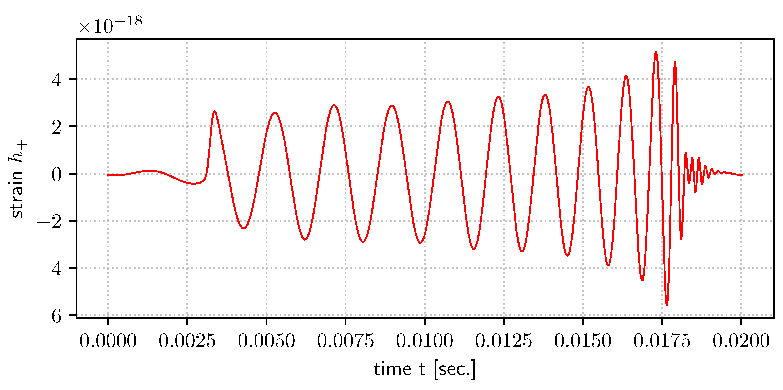
\includegraphics[width=0.5\textwidth]{figures/Capitolo_1/SHT2.2.pdf}
	\end{center}
	\vspace{-10pt}
	\caption{Forma d'onda per la coalescenza di una BNS con equazione di stato SHT2, in cui le masse sono tali da portare il sistema a collassare immediatamente in un BH, producendo nella fase di post merger il ringdown}
	\label{fig:FormaOndaBH}
	\vspace{-50pt}
\end{wrapfigure}
La formazione diretta di un buco nero dopo la coalescenza implica, come si osserva in figura \ref{fig:FormaOndaBH} lo spegnimento del segnale, con un collasso quasi sferico che genera delle onde gravitazionali minime\cite{sarin2020evolution}.

Questo tipo di segnale ha la particolarità, al contrario degli altri casi di post-merger, di ammattere uno studio analitico attraverso metodi perturbativi relativamente semplici (decrescita esponenziale con un tempo caratteristico legato alla massa del buco nero)\cite{maggiore2018gravitational}.

\subsection{Formazione di una NS ipermassiva}
\label{subsection:ipermassiva}	
La maggior parte delle coalescenze di stelle di neutroni porta alla formazione di stelle di neutroni ipermassive, supermassive o stabili. 

Una stella di neutroni ipermassiva è tale da avere una massa superiore al massimo in massa per una stella rotante uniformemente $M_{TOV}$, ma non collassa per la rotazione differenziale, cioè il fenomeno per cui le sue diverse parti ruotano con velocità angolare differente che permette una maggiore stabilità rispetto a stelle non rotanti o rotanti uniformemente \cite{Baumgarte_2000}, e per il supporto di gradienti termici.

\begin{wrapfigure}{r}{0.45\textwidth}
	\vspace{-35pt}
	\begin{center}
		\includegraphics[width=0.5\textwidth]{figures/Capitolo_1/SHT2.0.pdf}
	\end{center}
	\vspace{-10pt}
	\caption{Forma d'onda per la coalescenza di una BNS con equazione di stato SHT2, in cui le masse sono tali da portare il sistema a formare una NS ipermassiva, producendo nella fase di post merger un segnale visibile}
	\label{fig:FormaOndaToNS}
	\vspace{-30pt}
\end{wrapfigure}
Nel momento in cui la stella rallenta la sua rotazione e/o si raffredda, il supporto alla sua stessa massa termina e la stella collassa in un buco nero. 
Nel caso in cui la stella ipermassiva abbia massa tale che $M \gtrsim 1.2 M_{TOV}$ la rotazione uniforme non può dare sufficiente supporto centrifugo per evitare il collasso, per cui la stella collassa non appena la rotazione differenziale termina.

È in generale molto complessa la fisica che regola il collasso dell'ipermassiva residua tuttavia assumendo che per il rilascio del lampo gamma sia necessario tale collasso in buco nero, il ritardo con il quale si è osservato per GW170817, come si vedrà nel capitolo \ref{chapter:gw170817}, può essere, almeno in parte, spiegato con il collasso.


L'emissione di GW dalla fase di post-coalescenza è attesa avere una quantità di energia rilasciata sotto forma di GW relativamente ampia e confrontabile con il massimo dell'inspiral\cite{sarin2020evolution}. 

\subsection{Formazione di una NS con lunga vita media}
\label{subsection:long_lived}
I residui del post-merger che hanno una massa inferiore a $\smallsim1.2M_{TOV}$ sopravvivono per un tempo superiore al secondo e vengono denomiate supermassive se hanno una massa superiore al limite definito in precedenza $M_{TOV}$, mentre per valori inferiori sono stabili.
È importante osservare in figura \ref{fig:EvoluzioneBNS} che per entrambi i prodotti finali si passa comunque per una fase di forte rotazione differenziale immediatamente successiva alla coalescenza rendendo i metodi di ricerca di segnali di GW non differenti da quelli per il caso di residuo ipermassivo.
L'osservazione sperimentale mostra che questo tipo di esito si presenta in un numero non trascurabile di casi.

Come detto, le simulazioni mostrano che per stelle supermassive generate dalla coalescenza di un sistema binario di stelle di neutroni hanno una vita compresa tra $\smallsim10$s e $\smallsim10^4$s. In realtà l'osservazione sperimentale mostra che queste stelle tendono a collassare in una scala di tempi più breve di quella attesa e tale discrepanza si pensa possa includere eccessi di energia emessa in onde gravitazionali nelle prime fasi, o quark liberi che portano a modifiche nel momento di inerzia della stella rispetto al caso con materia ordinaria.

Questi vincoli hanno grande importanza, soprattutto per la ricerca futura: il fatto che le stelle di neutroni nascenti siano composte da quark non confinati suggerisce che vi sia una transizione di fase adrone-quark dipendente dalla temperatura e, comprendere dove avvenga questa transizione nel diagramma di fase nucleare è un informazione chiave per dedurre informazioni sul comportamento della materia nucleare e di conseguenza sull'equazione di stato.
Il fatto, invece, che le NS supermassive rallentino la rotazione soprattutto a causa dell'emissione di GW ha importanti conseguenze per la dinamica della NS stessa e permette di avere vincoli sull'energia per ricostruire la natura dell'oggetto residuo nelle future analisi\cite{sarin2020evolution}.
%neutrino emissions, thermal evolution, dynamical evolution, elettromagnetic observations?

%DA CANCELLARE(?)[Per le NS a lunga vita si conoscono le emissioni elettromagnetiche, mentre per le emissioni di onde gravitazionali la conoscenza del fenomeno risulta ancora incompleta: non si conosce con certezza la gerarchia di importanza dei meccanismi, per quanto tempo rimangono attive o quanta energia viene emessa. Le tre principali instabilita rilevanti per la produzione di GW sono le instabilità di spin-flip, di bar-mode e r-mode.
%L'instabilità precessionale spin-flip, legata al cambiamento di rotazione di un oggetto rotante, porta la nascente NS ad essere un "rotatore ortogonale" e quindi un ottimo emettitore di GW.
%L'instabilità bar-mode si presenta in due varietà: dinamica, che è attiva nel primo secondo della vita della NS, e secolare, che ha maggiore importanza nel lungo periodo. 
%Infine gli r-mode, ovvero oscillazioni toroidali a bassa frequenza per le quali la forza di Coriolis è la "forza di ripristino"\cite{sarin2020evo5lution}.]

\section[Frequenze caratteristiche]{Frequenze caratteristiche di coalescenza e post-coalescenza}
\label{section:frequenze_caratteristiche}
\begin{wrapfigure}{r}{0.45\textwidth}
	\vspace{-15pt}
	\begin{center}
		\includegraphics[width=0.5\textwidth]{figures/Capitolo_1/GW_spectrogram_short_APR4-q10-M1300.pdf}
	\end{center}
	\vspace{-10pt}
	\caption{Forma d'onda e relativo spettrogramma per la coalescenza di una BNS con equazione di stato APR4 (morbida), \cite{Rezzolla_2016}}
	\label{fig:spettrogramma_merger_APR4}
	\vspace{-20pt}
\end{wrapfigure}
%Una BNS realistica presenta una massa compresa tra $\smallsim\SI{2.4}{\solarmass}$ e $\smallsim\SI{2.8}{\solarmass}$ e una differenza tra le due componenti che è di $\smallsim20\%$ o minore.
A partire dal segnale di GW, in particolare nelle fasi di coalescenza e post-coalescenza, possono essere ottenute informazioni sull'equazione di stato della materia a densità nucleare e, da un'analisi spettrale, informazioni sulla tidal deformability (deformabilità mareale) delle due stelle.

Simulazioni numeriche relativistiche di coalescenza di BNS e l'evoluzione della post-coalescenza mostra che l'emissione di GW da un residuo ipermassivo è legato alla EOS e può trovarsi a frequenze comprese tra $\smallsim2$ e 4kHz, ed è fortemente correlato con la compattezza e la deformabilità mareale delle stelle. Questa correlazione, con quantità calcolate per stelle di neutroni fredde e non rotanti, stato in cui non si trova l'ipermassiva residua, suggerisce come gli effetti dovuti a rotazione e temperatura giocano un ruolo limitato nelle proprietà del segnale di onda gravitazionale e mostra come la misura del modo dominante nella frequenza del post-merger possa portare a una importante misura dell'equazione di stato nucleare\cite{sarin2020evolution}.

\begin{wrapfigure}{r}{0.45\textwidth}
	\vspace{-15pt}
	\begin{center}
		\includegraphics[width=0.5\textwidth]{figures/Capitolo_1/GW_spectrogram_APR4-q10-M1300.pdf}
	\end{center}
	\vspace{-10pt}
	\caption{Forma d'onda e relativo spettrogramma per la post-coalescenza di una BNS con equazione di stato APR4, \cite{Rezzolla_2016}}
	\label{fig:spettrogramma_postmerger_APR4}
	\vspace{-30pt}
\end{wrapfigure}
Considerando dunque il segnale gravitazionale dovuto alla coalescenza di due stelle di neutroni, con una differneza di massa inferiore a 20\%, \cite{Rezzolla_2016} ne riassume le proprietà spettrali fondamentali in:
\begin{itemize}
	\item la frequenza della GW al massimo di ampiezza $f_{max}$ è legata in modo quasi-universale con la tidal deformability delle due stelle;
	\item le frequenze $f_1$, $f_{2,i}$ e $f_3$ rappresentano i picchi principali visibili dall'osservazione del post-merger, tra le quali si ottiene la seguente relazione empirica:
	\begin{equation}
	f_{2,i}\simeq\frac{f_1 + f_3}{2} 
	\label{eqn:f1_2_3}
	\end{equation} 
	il picco $f_1$ è legato alla compattezza delle stelle, mentre il picco $f_{2,i}$ è legato al raggio della configurazione non rotante più massiva e corrisponde al modo fondamentale della NS ipermassiva con l=2=m;
\end{itemize}

\begin{itemize}
	\item si identifica in alcuni casi un altro picco $f_{2-0}$ che si riferisce all'accoppiamento tra il modo fondamentale con l=2=m e il modo con simmetria assiale, cioè con l=2 e m=0;
	\item il picco $f_{spiral}$ associato alla deformazione spiraleggiante dovuta alla rotazione, è però impossibile da misurare in calcoli numerici e si utilizzano dunque i valori prodotti da considerazioni analitiche. Si nota infine che $f_{spiral}$ coincide per molte EOS (in particolare EOS rigide) con la frequenza $f_1$, mentre per altre (EOS morbide) non si ha questa corrispondenza.
\end{itemize}

Nella fase di post-merger, nei casi in cui il sistema non collassa immediatamente in un buco nero, evidenziando nella forma d'onda una fase di ringdown in cui il segnale si spegne, l'unica frequenza a sopravvivere è il picco $f_2$, spariscono gli altri picchi, lasciando solo $f_{2-0}$ a basse energie.

È poi possibile trovare diverse relazioni quantitative che legano le frequenze osservate con le proprietà stellari, che risultano particolarmente utili come verifica delle previsioni teoriche.

%	% !TEX root = ../../Tesi_Triennale_PMNS.tex
\chapter[Osservazione di GW da BNS]{GW170817: osservazione di onde gravitazionali prodotte da un sistema binario di stelle di neutroni}
\label{chapter:gw170817}
Rivelato il 17 Agosto 2017 dal network LIGO-Virgo, GW170817 è il primo segnale di onda gravitazionale generato dallo spiraleggiamento un sistema binario di stelle di neutroni.
Il segnale osservato, alla fine del secondo run di misure O2, è tutt'ora il più energetico osservato finora tra questi tipi di segnale, con un rapporto segnale su rumore (SNR) di 32.4.

Oltre al segnale di GW è stato osservato un gamma ray burst, dopo 1.7s dalla coalescenza.
\section{Osservazione dello spiraleggiamento}
\label{section:osservazioneInspiralGW170817}
\begin{wrapfigure}{r}{0.5\textwidth}
	\vspace{-15pt}
	\begin{center}
		\includegraphics[width=0.4\textwidth]{figures/Capitolo_2/gw170817_time_freq.png}
	\end{center}
	\vspace{-10pt}
	\caption{Segnali in una mappa tempo frequenza nel network di detectors, presa da \cite{Abbott_2017b}}
	\label{fig:osservazione_gw170817}
	\vspace{-40pt}
\end{wrapfigure}
La rappresentazione tempo-frequenza dei dati a cui viene sottratto il rumore e sbiancati. Si può notare immediatamente che il segnale che, idealmente deve presentare la forma di un chirp, è ben visibile nei due rivelatori LIGO, meglio in Livingston che in Hanford, mentre in Virgo, a causa della posizione celeste della sorgente del segnale, non è possibile distiguere nessun pattern dal rumore di fondo. La (non) rivelazione risulta comunque utile, soprattutto per permettere l'individuazione della posizione celeste della sorgente.

L'analisi del segnale mostra un segnale coerente nei due detector LIGO, grazie al quale si individua la sorgente in una regione identificata da un angolo solido di 31 $\text{deg}^2$, che a sua volta ha permesso l'identificazione della controparte elettromagnetica GRB170817A. 
Si è ottenuto inoltre un SNR combinato tra i detector di 32.4 che rendono questo segnale il più intenso rivelato finora.\cite{Abbott_2017b}

\subsection{Proprietà della sorgente}
\label{subsection:proprietàSorgGW170817}
La relatività generale fa previsioni abbastanza dettagliate sull'evoluzione della frequenza, che è legato, nella prima fase, a una combinazione delle masse delle stelle progenitrici, detta massa di chirp 
\begin{equation}
	\mathcal{M} = \frac{(m_1m_2)^{3/5}}{(m_1+m_2)^{1/5}}
	\label{eqn:chirpmass}
\end{equation}
Nelle fasi più avanzate, le orbite si stringono e aumenta la frequenza dell'onda gravitazionale, mentre la fase della GW è sempre più influenzata da effetti relativistici legati al rapporto tra le masse $q = m_2/m_1$ e dagli accoppiamenti spin-orbita e spin-spin. 
La composizione interna degli oggetti diventa importante quando la distanza tra essi diventa paragonabile alle dimensioni dell'oggetto stesso. 

Le proprietà della sorgente di onde gravitazionali sono ottenute dal confronto con le forme d'onda predette dalla teoria. Viene fatta dunque una analisi Bayesiana nel range di frequenze 30-2048Hz che include gli effetti dell'incertezza di calibrazione di $1\sigma$ sul segnale ricevuto.

La sorgente viene in questo modo identificata in una regione celeste di 28$\text{deg}^2$ di area e $380\text{Mpc}^3$ di volume, utilizzando una combinazione di timing, fase e ampiezza dei tre detector. La distanza luminosa, la più prossima osservata finora, viene individuata in $40_{-14}^{+8}$Mpc. Per le masse delle stelle compatte risulta più semplice dedurre la massa di chirp, indipendente dalla scelta della prior nell'analisi Bayesiana, che si valuta in $\mathcal{M}=1.188_{-0.002}^{+0.004}$, rispetto alle masse singole, che soffrono invece della degenerazione tra il rapporto tra le masse $q$ e le componenti dello spin $\chi_1$ e $\chi_2$. È necessario fare quindi assunzioni a partire dalle EOS che si considerano, ottenendo dei range $m_1 \in (1.36, 2.26)M_\odot$ e $m_2 \in (0.86, 1.36)M_\odot$ evidentemente meno precisi, ma comunque utili come evidenza della natura di stelle di neutroni del sistema binario, escludendo invece la possibilità di buchi neri che prevederebbe range di masse superiori\cite{Abbott_2017b}.

QUALCOSA SULLE TIDAL DEFORMABILITIES?
\section{Ricerca del post-merger del residuo}
\label{section:postmergerGW170817}
L'analisi del post-merger, atteso in seguito all'osservazione del segnale GW170817, non ha portato ad evidenza statisticamente significativa di un oggetto in seguito alla coalescenza, ma ha permesso di ottenere informazioni sul limite superiore sulle ampiezze di strain ed energie di GW osservabili. Gli attuali detector infatti non sono calibrati in modo tale da permettere rivelazioni alle alte frequenze del post-merger.

Mentre lo studio del segnale elettromagnetico associato alla GW non permette di escludere nessuno dei possibili stati finali indicati in sezione \ref{section:residual}, grazie ai valori ottenuti per le masse dei progenitori date nella sezione \ref{subsection:proprietàSorgGW170817} si calcola che per un ampio range di equazioni di stato la coalescenza produce uno stato di NS ipermassiva. Questo spiega anche il ritardo del lampo-$\gamma$rispetto all'istante di rivelazione del segnale di merger. 

\begin{wrapfigure}{r}{0.5\textwidth}
	\vspace{-15pt}
	\begin{center}
		\includegraphics[width=0.5\textwidth]{figures/Capitolo_2/noiseData.png}
	\end{center}
	\vspace{-5pt}
	\caption{Sensibilità di ciascun rivelatore durante il run O2, indicata dall'ampiezza del rumore di strain in funzione della frequenza, presa da \cite{Abbott_2019}}
	\label{fig:NoiseFrequenze}
	\vspace{-10pt}
\end{wrapfigure}
Come si vedrà nella sezione \ref{section:analisiSimSingole} in base alla EOS che si considera si ottiene un contributo diverso nel post-merger che inizia attorno a $\smallsim1$kHz. Più in generale, oltre alla EOS hanno fondamentale importanza le masse e gli spin degli oggetti iniziali. 
Per quanto riguarda invece la rivelazione di questa fase del segnale, anche considerando modelli ottimistici da stati finali di NS ipermassiva o supermassiva, l'SNR atteso per distanze di $\smallsim40$Mpc è $\smallsim1-2$ ordini di grandezza più piccolo di quello rivelabile dal network LIGO-Virgo attualmente utilizzato, facendo uso di algoritmi di confronto con segnali modellati (che comunque sono meno utilizzati per il post-merger, per la difficoltà nel modellare questa fase del segnale).
Si ipotizza tuttavia che nei prossimi run O3-O4 la sensibilità del network sarà tale da permettere la rivelazione di queste emissioni.

Come si può osservare in figura \ref{fig:NoiseFrequenze} i tre detector del network hanno zone diverse di sensibilità, in particolare si nota che in generale la sensibilità diminuisce significativamente ad alte frequenze. Il rumore di LIGO Hanford è più alto rispetto a Livingston nella banda di frequenza compresa tra 100Hz e 1kHz, mentre Virgo ha sofferto grandi fluttuazioni di rumore e proprietà spettrali non stazionarie a frequenze superiori a 2.5kHz.

Per l'analisi sono stati usati due diversi algoritmi, in base al tipo di segnale ricercato: per segnali di brave durata è stato usato cWB (Coherent Wave Burst) utilizzando i dati di LIGO tra 1024Hz e 4096Hz, mentre per i segnali di durata intermedia si è utilizzato l'algoritmo STAMP (Stochastic Transient Analysis Multidetector Pipeline) nelle frequenze comprese tra 24Hz e 2000Hz e tra 2000Hz e 4000Hz nei dati di LIGO, mentre cWB con i dati del network LIGO-Virgo ricerca le frequenze tra 24Hz e 2048Hz. 

Per la ricerca di segnali con incertezze teoriche cosi grandi l'utilizzo di metodi di ricerca matched-filtering, ovvero un metodo che utilizza segnali di forme conosciute e attraverso funzioni di filtraggio si esclude la componente di rumore, in particolare si sceglie la funzione che massimizza il rapporto segnale su rumore (SNR) per tale segnale\cite{maggiore2008gravitational}. È immediato comprendere che non conoscendo con certezza la forma che deve assumere il segnale questo metodo risulta inefficace per la ricerca del post-merger. Gli algoritmi che si usano ricercano eccessi di potenza in una mappa tempo-frequenza e usando metodi di riconoscimento dei pattern si può identificare la presenza di segnali di GW nelle mappe. In particolare gli algoritmi sono tali da considerare i dati del network e non dei singoli rivelatori, utilizzando tecniche che permettono di combinare coerentemente i dati dei singoli detector e dare risposte differenti a forme d'onda diverse.

Come anticipato, la ricerca viene divisa tra segnali brevi ($\lesssim$1s) e intermedi ($\lesssim$500s).
\subsection{Segnali brevi}
L'analisi dei segnali brevi, ad alte frequenze viene fatta con l'algoritmo cWB e consistono nella ricerca di eccessi di potenza nell'intervallo di 2s che precede il segnale elettromagnetico GRB 170817a, che comprende quindi anche il merger.
In particolare l'algoritmo valuta la massima verosimiglianza di eccessi di potenza in una trasformata di wavelet a multi-risoluzione per ogni detector, classificando gli eventi in una gerarchia di SNR. La significanza degli eventi è data dal confronto con la distribuzione del fondo stocastico, che è generata con metodi che saranno precisati nel capitolo \ref{chapter:cwb}. 

È convenzione esprimere la sensibilità della ricerca di una data forma d'onda in $h_{rss}^{50\%}$, ovvero la somma in quadratura delle ampiezze di strain di segnali che sono rivelati con un'efficienza del 50\%. La quantità $h_{rss}$ è definito come
\begin{equation}
	h_{rss} = \sqrt{2\int_{f_{min}}^{f_{max}}df(|\tilde{h}_+(f)|^2 + |\tilde{h}_\times(f)|^2 )}
\end{equation}
dove $f_{min}$ e $f_{max}$ sono rispettivamente le frequenze massima e minima sulle quali si effettua la ricerca. 
Il criterio su $h_{rss}^{50\%}$ scelto per questo metodo di ricerca è tale da avere una probabilità di falso allarme di $10^{-4}$

Per evitare la possibile perdita di segnali di EOS rigide, si fa la scelta conservativa di ricercare segnali a partire da 1024Hz, nonostante tutte le forme d'onda hanno emissioni dominanti molto al di sopra di tale soglia.

In conclusione, non viene trovata evidenza di nessun segnale di GW in questa banda di frequenze.
L'ampiezza di strain per produrre una probabilità del 50\% di rivelazione di un segnale è compresa tra $2.1 x 10^{-22} \text{Hz}^{-1/2}$ e $3.5 x 10^{-22} \text{Hz}^{-1/2}$. L'energia irradiata da un sorgente che emette isotropicamente è data da 
\begin{equation}
	E_{gw}^{iso} = \frac{\pi c^3}{2G}\mathcal{D}^2\int d\Omega \int_{f_{min}}^{f_{max}}dff^2(|\tilde{h}_+(f)|^2 + |\tilde{h}_\times(f)|^2 ) \approx \frac{\pi^2 c^3}{G}\mathcal{D}^2\bar{f}^2h_{rss}^2
\end{equation}
con $\mathcal{D}$ è la distanza dalla sorgente e $\bar{f}$ è la frequenza caratteristica data da 
\begin{equation}
	\bar{f} = \frac{2}{h_{rss}^2}\int_{f_{min}}^{f_{max}}dff(|\tilde{h}_+(f)|^2 + |\tilde{h}_\times(f)|^2 )
\end{equation}

In questo modo si ottiene un range di energie rivelabili secondo il criterio del $h_{rss}^{500\%}$ è dato da $4.8-\SI{19.6}{\solarmass}c^2$, al di fuori delle masse in gioco per BNS, per cui non è possibile con i rivelatori attuali rivelare le emissioni di GW di NS ipermassive associate a GW170817.
\subsection{Segnali di durata intermedia}
Per segnali di durata intermedia si utilizzano i due algoritmi cWB e STAMP, concentrando la ricerca in una zona limitata dello spazio, indicata dalla controparte elettromagnetica che permette di evitare trigger accidentali.

\begin{wrapfigure}{r}{0.5\textwidth}
	\vspace{-15pt}
	\begin{center}
		\includegraphics[width=0.5\textwidth]{figures/Capitolo_2/signal.png}
	\end{center}
	\vspace{-5pt}
	\caption{\cite{Abbott_2017b}}
	\label{fig:signalInspiral}
	\vspace{-10pt}
\end{wrapfigure}
\section{Sugli altri eventi rivelati}
\subsection*{title}
%Breve rassegna dei metodi di rivelazione: stamp \& cwb

non trovato alcun segnale\cite{Abbott_2017a}
%	% !TEX root = ../../Tesi_Triennale_PMNS.tex
\chapter[cWB]{cWB: proprietà dell'algoritmo per la rivelazione e la ricostruzione di segnali di onde gravitazionali}
\label{chapter:cwb}
I metodi coerenti le statistiche vengono calcolate come somma coerente delle risposte dei detector singoli. Gli algoritmi che sfruttano questi metodi devono risultare più efficienti, devono cioè avere una probabilità di falso allarme più bassa, rispetto alle statistiche calcolate sulle risposte di ogni detector singolarmente.

L'algoritmo che si utilizza, Coherent WaveBurst (cWB), differisce dai metodi tradizionali che identificano gli eventi nei detector singolarmente usando statistiche di eccesso di potenza e poi verificano la coerenza tra i segnali nei vari detector. Esso utilizza infatti i dati di tutti i detector in un'unica statistica coerente costituita da una analisi della massima likelihood. 
I vantaggi di questo tipo di analisi sono molteplici: innanzitutto la sensibilità del metodo non sarà limitata dal detector meno sensibile nel network, in quanto la likelihood utilizzata nei metodi coerenti rappresenta il rapporto segnale su rumore (SNR) totale del segnale ricostruito/rivelato dal network. Inoltre questo metodo permette di costruire altre statistiche coerenti, come il null stream o il coefficiente di correlazione  del network, per distinguere segnali che effettivamente hanno una controparte fisica rispetto a eccessi di rumore ambientale o strumentale. Infine è possibile ricostruire la posizione celeste della sorgente\cite{Klimenko_2008}.

L'algoritmo cWB lavora in due modi differenti: viene utilizzato in tempo reale con i dati provenienti dai rivelatori per identificare e ricostruire candidati significativi e poter, una volta ottenuta una prima stima della posizione celeste della sorgente, condividerla con i telescopi partner per identificare i segnali elettromagnetici legati; alternativamente si utilizza per l'analisi di dati consolidati volta a ottenere risultati più approfonditi sull'evento, stabilendo la significanza degli eventi osservati e identificando le stelle progenitrici\cite{Klimenko_2016}. In questo e nel prossimo capitolo ci si concentrerà sul secondo tipo di analisi.
\section{Analisi coerente}
\label{section:coherent_analysis}
La pipeline di cWB per rivelare e ricostruire segnali utilizza un metodo basato sul funzionale rapporto di verosimiglianza, che, in un'ipotesi idealistica di rumore gaussiano quasi stazionario, può essere scritto nel dominio di wavelet (in un piano tempo-frequenza) come
\begin{equation}
	\mathcal{L} = \sum_{k=1}^{K}\sum_{i,j=1}^{N}\left(\frac{w_k^2[i,j]}{\sigma_k^2[i,j]} - \frac{(w_k[i,j]-\xi_k[i,j])^2}{\sigma_k^2[i,j]}  \right)
	\label{eqn:Likelihood}
\end{equation}
dove K è il numero di detector nel network, $w_k[i,j]$ è il campione di dati del detector (l'indice i itera sui tempi, mentre l'indice j itera sulle frequenze) e infine $\xi_k[i,j]$ è la risposta del detector k-esimo.
Il rumore del detector è è caratterizzato dalla deviazione standard $\sigma_k[i,j]$ che può variare lungo il piano tempo-frequenza.
Le risposte del network sono scritte come
\begin{equation}
	\xi_k[i,j] = F_{+,k}h_+[i,j] + F_{\times,k}h_\times[i,j]
	\label{eqn:detector_response}
\end{equation}
dove $h_{+}[i,j]$ e $h_{\times}[i,j]$ sono le ampiezze delle due polarizzazioni della GW e $F_{+,k}(\theta,\phi)$ e $F_{\times,k}(\theta,\phi)$ sono gli antenna pattern del detector k-esimo\cite{Klimenko_2008}. Gli antenna pattern descrivono come il detector riceve l'energia in funzione della posizione angolare. *Breve descrizione antenna pattern* *immagine antenna pattern di uno dei rivelatori*\cite{Schutz_2011}.

Dunque, al variare di $h_{+}[i,j]$ e $h_{\times}[i,j]$ varia anche $\mathcal{L}$, l'obiettivo è quindi ottenere i valori delle ampiezze che massimizzano il funzionale di verosimiglianza e quindi si deduce la forma d'onda nel dominio dei tempi facendo una trasformazione di wavelet inversa.%, che consisterà dunque 

Per semplicità si introducono i seguenti vettori:
\[
	\textbf{w}[i,j] = \left(\frac{w_1[i,j]}{\sigma_1[i,j]},\dots, \frac{w_K[i,j]}{\sigma_K[i,j]} \right) ;
	\quad
	\textbf{f}_{+(\times)}[i,j] = \left(\frac{F_{1+(\times)}[i,j]}{\sigma_1[i,j]},\dots, \frac{F_{K+(\times)}[i,j]}{\sigma_K[i,j]} \right) 
\]
mentre con la notazione $\sum_{\Omega_{TF}} = \sum_{i,j=1}^N$, in quanto si scriverà $\Omega_{TF}$ come il dominio tempo-frequenza. 

Il funzionale rapporto di verosimiglianza in equazione \ref{eqn:Likelihood} si può scrivere come
\begin{equation}
	\mathcal{L} = \mathcal{L}_+ + \mathcal{L}_\times = \sum_{\Omega_{TF}}\left[ \textbf{w} \cdot \textbf{f}_+ - \frac{1}{2}|\textbf{f}_+|^2h_+^2\right] + \sum_{\Omega_{TF}}\left[ \textbf{w} \cdot \textbf{f}_\times - \frac{1}{2}|\textbf{f}_\times|^2h_\times^2\right]
	\label{eqn:label_separated}
\end{equation}
dove i vettori di antenna pattern $\textbf{f}_+$ e $\textbf{f}_\times$ sono definiti nel Dominant Polarisation wave Frame (DPF), ovvero il piano in cui entrambi gli antenna pattern sono reali e definiti positivi e vale $\textbf{f}_+ \cdot \textbf{f}_\times = 0$. Alla luce di questo per ottenere la massima likelihood si dovrà risolvere le equazioni:
\begin{equation}
	\textbf{w} \cdot \textbf{f}_+ = |\textbf{f}_+|^2h_+ \quad\quad\quad  \textbf{w} \cdot \textbf{f}_\times = |\textbf{f}_+|^2h_\times 
	\label{eqn:sistema_soluzione}
\end{equation}
\paragraph{Regolatori} C'è una particolare classe di vincoli, i regolatori, che dipendono da come il network reagisce a un determinato segnale\cite{Klimenko_2008}.
\section{Algoritmi per l'analisi dati}
\subsection{Trasformazioni di wavelet}
\label{subsection:wavelet_transform}
\begin{wrapfigure}{r}{0.46\textwidth}
	\vspace{-35pt}
	\begin{center}
		\includegraphics[width=0.475\textwidth]{figures/Capitolo_3/L1_scalogram_0.png}
	\end{center}
	\vspace{-5pt}
	\caption{Scalogramma ottenuto da una analisi di una simulazione di coalescenza di una BNS con EOS SHT2.0 con rumore gaussiano del detector LIGO Hanford}
	\label{fig:scalogram_example}
	\vspace{-40pt}
\end{wrapfigure}
Le trasformazioni di wavelet, partendo dai dati discreti, producono serie di dati $w[i,j]$ nel piano tempo-frequenza. Lo spettro di wavelet può essere quindi rappresentato con uno scalogramma tempo-frequenza. La risoluzione nel dominio del tempo $\Delta t_j(R)$ è determinata dal rate di campionamento R e dall'indice di scala j. Poiché le trasformazioni di wavelet costituiscono una serie di trasformazioni di Fourier infinitesime, conservano il volume del campione, pari a 1/2 per la serie temporale in input. Si avrà quindi una risoluzione in frequenza $\Delta f_j$ definita come 1/(2$\Delta t_j$) che determina la larghezza di banda per l'indice j. Per ottimizzare la ricerca nel piano, cWB procede con diverse trasformazioni a risoluzioni diverse, che permette di ottenere il grafico in figura \ref{fig:scalogram_example}.
\subsection{Filtro di predizione lineare dell'errore}
\label{subsection:lpe_filter}
I filtri per la predizione lineare dell'errore (LPE) sono usati per rimuovere le componenti prevedibili dalla serie temporale in input. Possono essere applicati nel dominio di wavelet, ma più frequentemente vengono usati nel dominio temporale restituendo una serie temporale sbiancata.

Ogni layer di wavelet (quindi a frequenza fissata) è una serie temporale, quindi anzichè applicare il filtro LPE alla sere temporale $x(t)$, si può fare prima una decomposizione di wavelet $x(t)\rightarrow w(f,t)$ e quindi applicare il filtro ad ogni layer di wavelet. Si ottiene dunque un campione $w'(f, t)$ da cui è possibile ricostruire la serie temporale sbiancata $x'(t)$ attraverso una trasformazione di wavelet inversa\cite{Klimenko_2008}.
\subsection{Filtri per il ritardo temporale nel dominio di wavelet}
\label{subsection:time_delay_filters}
Per la valutazione della likelihood è necessario computare il prodotto scalare $\bra{x_n(\tau_n)}\ket{x_m(\tau_m)}$, dove bisogna considerare un ritardo intrinseco del set di dati del rivelatore $n$ rispetto a $m$, in quanto le GW viaggiano a velocità finita pari a $c$. Dunque il ritardo temporale $\tau_n - \tau_m$ dipende dalla posizione $(\theta, \phi)$ della sorgente.

Nel dominio di wavelet è invece necessario calcolare il prodotto interno $\bra{w_n(\tau_n)}\ket{w_m(\tau_m)}$, le ampiezze ritardate possono essere calcolate a partire dalle ampiezze originali utilizzando un filtro di ritardo temporale $D_{kl}(\tau)$
\begin{equation}
	w_{n,m}(i,j,\tau) = \sum_{kl}D_{kl}(\tau, j)w_{n,m}(i+k, j+l)
	\label{eqn:time_filter}
\end{equation}
dove $k$ ed $l$ sono le coordinate locali nel piano tempo-frequenza rispetto alla posizione $(i,j)$.

La costruzione di questi filtri è legata alla decomposizione delle funzioni di wavelet ritardate $\Psi_j(t+\tau)$ nella base delle funzioni non traslate $\Psi_j(t)$. Si procede dunque per step:
\begin{enumerate}
	\item viene creata una serie di wavelet con un solo coefficiente pari all'unità nella posizione $(i,j)$;
	\item viene applicata la trasformazione di wavelet inversa ricostruendo $\Psi_j(t)$ nel dominio dei tempi;
	\item viene applicata la traslazione temporale $\Psi_j(t)\rightarrow\Psi_j(t+\tau)$ e si decompone quest'ultima;
	\item le ampiezze di wavelet ottenute nelle posizioni $(i+k, j+l)$ rappresentano i coefficienti del filtro $D_{kl}(\tau, j)$ per il layer j.
\end{enumerate}
L'applicazione di questo filtro porta a una perdita di energia, valutabile in $\epsilon_K = 1 - \sum_{K}D_{kl}^2$
%\begin{equation}
%	\epsilon_K = 1 - \sum_{K}D_{kl}^2
%	\label{eqn:energy_loss}
%\end{equation}
e perciò la lunghezza del filtro sarà legata alla quantità di energia acsecettabile da perdere (valori tipici sono $K>20$ per ottenere una perdita di energia inferiore a $1\%$)\cite{Klimenko_2008}.
\subsection{Generazione di trigger coerenti}
\label{section:coherent_trigger}
La generazione dei trigger, quindi l'identificazione dei segnali, è basata su statistiche di eccesso di potenza e di correlazione incrociata tra i segnali dei detector. 

Il funzionale di likelihood viene calcolato come somma sui campioni selezionati per l'analisi, il numero di termini sommati sipende all'area nel piano tempo-frequenza che si considera, se tale somma consiste di un solo elemento si può scrivere il funzionale come
\begin{equation}
	\mathcal{L}_p(i,j,\theta,\phi)=|\textbf{w}|^2 -|\textbf{w} - \textbf{f}_+h_+ - \textbf{f}_\times h_\times|^2
	\label{eqn:likelihood_single_term}
\end{equation}
Poiché è possibile applicare il metodo della likelihood al funzionale \ref{eqn:likelihood_single_term}, si può trovare il massimo $L_p(\theta, \phi)$ al variare di $h_+$ e $h_\times$ e quindi ricercare il massimo in funzione della posizione celeste
\begin{equation}
	L_m(i,j)= \max_{\theta, \phi}[L_p(i,j,\theta,\phi)]
	\label{eqn:max_L}
\end{equation}
\begin{wrapfigure}{r}{0.46\textwidth}
	\vspace{-20pt}
	\begin{center}
		\includegraphics[width=0.475\textwidth]{figures/Capitolo_3/l_tfmap_scalogram.png}
	\end{center}
	\vspace{-5pt}
	\caption{Mappa di Likelihood ottenuta da una analisi di una simulazione di coalescenza di una BNS con EOS SHT2.0 con rumore gaussiano del network LIGO-Virgo}
	\label{fig:Likelihood_example}
	\vspace{-10pt}
\end{wrapfigure}
La statistica $L_m$ ha quindi il significato della massima energia rivelata dal network in una determinata posizione del piano tempo-frequenza. Selezionando quindi I valori di $L_m$ sopra una determinata soglia si può identificare un cluster di pixel come potenziale segnale di GW. In questo modo si identificano i segnali combinando i dati dell'intero network e non si cercano i segnali sui singoli detector, verificando successivamente la coerenza.
A questo punto si devono ricostruire i parametri del segnale legato al trigger incluse la posizione della sorgente, le due polarizzazioni della GW, le risposte individuali dei rivelatori e le statistiche di massima likelihood dei trigger. In particolare la likelihood è ricostruita come
\begin{equation}
	\mathcal{L}_c(\theta,\phi) = \sum_{i,j}\mathcal{L}_p(i,j,\theta, \phi)
\end{equation}
La massima likelihood $L_{max}$ è ottenuta facendo variare $L_c$ su $\theta$ e $\phi$ ed è calcolata su tutti i pixel di likelihood nel piano tempo frequenza per formare il trigger coerente\cite{Klimenko_2008}.
\section{Selezione dei trigger coerenti}
Nel caso di rumore gaussiano stazionario la massima verosimiglianza è l'unica statistica necessaria per la rivelazione e per la selezione degli eventi, per cui la probabilità di falso allarme e di scartare eventi effettivi è legata alla soglia minima per $L_{max}$. Nella realtà tuttavia il rumore non è tale, ma i dati sono sporcati da rumore strumentale e ambientale, per cui è necessario applicare altri metodi per distinguere i segnali reali. Alcuni esempi, utilizzati da cWB sono le statistiche coerenti ricavate dalle matrici di verosimiglianza e null
La matrice di likelihood $L_{mn}$ è ottenuta dalla forma quadratica della likelihood
%da completare la parte dei regolatori a cui questa parte fa riferimento.
\begin{equation}
	L_{max} = \sum_{mn}L_{mn} = \sum_{mn}\left[\left< w_nw_me_{+n}e_{+m} \right> + \left< w_nw_me'_{\times n}e'_{\times m} \right>\right]
	\label{eqn:likelihood_matrix}
\end{equation}
dove $m\text{ e }n$ sono gli indici che identificano i detector. Gli elementi della diagonale di $L_{mn}$ descrivono l'energia incoerente normalizzata, mentre quelli dell'antidiagonale sono espressione dell'energia coerente normalizzata, la cui somma restituisce l'energia coerente totale $E_{coh}$ rivelata dal network. Si può dunque esprimere i coefficienti di correlazione per detector allineati e quindi l'energia coerente ridotta
\begin{equation}
	r_{mn} = \frac{L_{mn}}{\sqrt{L_{nn}L_{mm}}} \quad\quad\quad \rightarrow \quad\quad\quad e_{coh}=\sum_{mn}L_{nm}|r_{nm}|, \quad n\neq m
	\label{eqn:coherent_energy}
\end{equation}
quest'ultima in particolare risulta uno dei parametri più efficienti per l'accettazione/rifiuto di un trigger.

La matrice di null rappresenta l'energia normalizzata del rumore ricostruito
\begin{equation}
	N_{nm} = E_{nm}-L_{nm}
\end{equation}
con $E_{mn}$  è la matrice diagonale delle energie normalizzate dei detector $E_{mm}  = \left<x_m^2\right>$. Per distinguere i segnali effettivi da rumore strumentale e ambientale si usano i coefficienti di correlazione 
\begin{equation}
	C_{net} = \frac{E_{coh}}{N_{ull}+|E_{coh}|}, \quad\quad\quad c_{net} = \frac{e_{coh}}{N_{ull}+|e_{coh}|}
\end{equation}
dove $N_{ull}$ è la somma di tutti gli elementi della matrice null, che rappresenta l'energia totale nella serie null. Accade infatti che eccessi di rumore vengano ricostruiti come segnale: i coefficienti $C_{net}$ e $c_{net}$ sono usati quindi come verifica della consistenza del segnale in quanto comparano l'energia del null e l'energia coerente\cite{Klimenko_2008}.
%Introduzione sull'algoritmo fatta nel paragrafo precedente, magari riprenderla veltocemente.
%Coherent analysis, significato e descrizione della likelihood: spiega quindi bene la differenza con gli algoritmi classici di confronto con segnali già modellati.

%regolatori, antenna pattern 

%algoritmi utilizzati: wavelet transformation, (linear predicion error), mappa verosimiglianza, mappa energia coerente (con piccoli grafici esemplificativi)

%(cenni sulla trasformazione di fase)


%\lipsum[3]\cite{Abbott_2017a}.
%
%\lipsum[4]\cite{Klimenko_2008}.
%
%\lipsum[6]\cite{Klimenko_2016}.

\section{Esempi di analisi utilizzando cWB}
\label{section:examples}

%\begin{center}
%	\begin{figure}[ht]
%		\centering
%		\includegraphics[scale=0.25, angle=0]{figures/Capitolo_3/noiseO4.pdf}
%		\setlength{\belowcaptionskip}{-20pt}
%		\caption{Prospetti \cite{Abbott_2020a}}
%		\label{fig:noiseO4}
%	\end{figure}
%\end{center}
%	% !TEX root = ../../Tesi_Triennale_PMNS.tex
\chapter{Analisi}
\label{chapter:analisi}
%\begin{wrapfigure}{r}{0.4\textwidth}
%	\vspace{-10pt}
%	\begin{center}
%		\includegraphics[width=0.3\textwidth]{figures/Capitolo_3/noiseO4.pdf}
%	\end{center}
%	\vspace{-5pt}
%	\caption{Sensibilità del network}
%	\label{fig:sensitivity_O4}
%	\vspace{-10pt}
%\end{wrapfigure}
Verrà presentata in questo capitolo un'analisi basata su un grande numero di forme d'onda iniettate in posizioni celesti generiche e ricostruite con cWB. Nella prima parte verrà fatta l'analisi delle curve di sensibilità e degli overlap, mentre la seconda parte sarà un'analisi volta a stimare sistematicamente la frequenza del post-merger, in particolare utilizzato sulle EOS APR4 e SHT2.
Le simulazioni utilizzano stime intermedie per le sensibilità che raggiungerà il network LIGO-Virgo nel run O4, non si considera invece il detector Kagra, nonostante sia previsto il suo utilizzo ben prima.

\section{Esempi di analisi utilizzando cWB}
\label{section:examples}
Vengono ora riportati alcuni esempi di analisi di eventi simulati utilizzando cWB, partendo da forme d'onda simulate a partire da due diverse EOS. 
%In particolare per ogni analisi verranno riportati i seguenti grafici e coefficienti:
%\begin{itemize}
%		\item il 
%		\item i grafici dell'ampiezza di strain ricostruita nel dominio dei tempi e nel dominio delle frequenze relative a un solo rivelatore.		
%\end{itemize}
\subsection{Equazione di stato APR4}
\label{subsection:APR4}
\begin{minipage}[c]{0.55\textwidth}
	Si riportano i principali coefficienti per identificare l'evento: il rapporto segnale su rumore (SNR); il valore del coefficiente $\rho$, ovvero una ranking statistic che esprime la significanza del segnale descrivendo l'ampiezza correlata effettiva; il coefficiente $c_{net}$ descritto in equazione \ref{eqn:coefficient_energy}; ED che descrive lo sbilanciamento dell'energia tra i detector nel network e, infine, $\theta$ e $\phi$ che descrivono la posizione celeste della sorgente;
\end{minipage}
\hspace{5mm}
\begin{tabular}{cccccc}
	\toprule
	SNR	&$\rho$	&$c_{net}$	&ED	&$\theta$	&$\phi$	\\
	\midrule
	103.1	&50.8	&0.97	&-0.1	&101.6	&-28.6	\\
	\bottomrule
\end{tabular}
\begin{figure}[H]
	\vspace{-20pt}
	\centering
	\subfloat[][\emph{LIGO-Livingstone}]
	{\includegraphics[width=.318125\textwidth]{figures/Capitolo_3/APR4_q09/L1_spectrogram_logy_0.png}} \quad
	\subfloat[][\emph{LIGO-Hanford}]
	{\includegraphics[width=.318125\textwidth]{figures/Capitolo_3/APR4_q09/H1_spectrogram_logy_0.png}} \quad
	\subfloat[][\emph{Virgo}]
	{\includegraphics[width=.318125\textwidth]{figures/Capitolo_3/APR4_q09/V1_spectrogram_logy_0.png}}
	\vspace{-5pt}
	\caption{Spettrogrammi per ciascun detector, che mostrano una rappresentazione sul piano tempo-frequenza del trigger, basandosi sulla scomposizione di Fourier}
	\label{fig:spettrogramma_apr4}
	\vspace{-15pt}
\end{figure}
Il segnale che si mostra è particolarmente energetico, perché è stato simulato ad una distanza molto ravvicinata ($d \simeq 1.25$Mpc). Si osservano quindi coefficienti particolarmente elevati.
Come si può osservare in Figura \ref{fig:spettrogramma_apr4}, mentre i detector LIGO-Livingstone e LIGO-Handford rivelano in modo evidente un segnale già ad un'analisi visiva, senza rumore significativo a sporcare la rivelazione, nella mappa di Virgo risulta distinguibile il segnale, tuttavia con rumore significativo e si può notare anche come guardando la scala di significanze del segnale questo risulti di un ordine di grandezza inferiore per Virgo, rispetto ai due rivelatori LIGO. Questo è probabilmente dovuto al fatto che i rivelatori LIGO sono allineati tra loro, mentre disallineati rispetto a Virgo e soprattutto alla posizione celeste della sorgente, favorevole ai primi due.

\begin{wrapfigure}{r}{0.46\textwidth}
	\vspace{-35pt}
	\begin{center}
		\includegraphics[width=0.475\textwidth]{figures/Capitolo_3/APR4_q09/l_tfmap_scalogram.png}
	\end{center}
	\vspace{-5pt}
	\caption{Mappa di verosimiglianza nel piano tempo-frequenza, che descrive il contributo dell'energia totale del campione associato all'evento ricostruito}
	\label{fig:Likelihood_APR4}
	\vspace{-10pt}
\end{wrapfigure}
Nel grafico della likelihood in figura \ref{fig:Likelihood_APR4}, si osserva una tipica figura a chirp, in cui la parte inferiore, a basse frequenze, rappresenta l'inspiral fino alla coalescenza, mentre il cluster di dati in alto, a frequenze particolarmente elevate ($\smallsim 3.3$KHz) corrisponde all'emissione del post-merger.
Infine nei grafici che seguono in figura \ref{fig:strain_apr4} si osservano le ricostruzioni della forma d'onda, in particolare in nero è plottato il segnale iniettato nella simulazione, mentre in rosso il segnale ricostruito. In particolare osservando il grafico delle frequenze si può notare come non sia stato ricostruito tra $\smallsim2.5$KHz e $\smallsim3$KHz, giustificando la separazione tra i cluster nel grafico della likelihood.
\begin{figure}[H]
	\vspace{-20pt}
	\centering
	\subfloat[][\emph{Dominio dei tempi}]
	{\includegraphics[width=.45\textwidth]{figures/Capitolo_3/APR4_q09/L1_wf_white_inj_rec.png}} \quad
	\subfloat[][\emph{Dominio delle frequenze}]
	{\includegraphics[width=.45\textwidth]{figures/Capitolo_3/APR4_q09/L1_wf_white_inj_rec_fft.png}}
	\vspace{-5pt}
	\caption{Ampiezza di strain ricostruita nel dominio dei tempi e nel dominio delle frequenze relative a un solo rivelatore}
	\label{fig:strain_apr4}
	\vspace{-15pt}
\end{figure}
\subsection{Equazione di stato SHT2}
\label{subsection:SHT2}
Per motivi di spazio non verranno presentate le analisi complete, come per l'equazione di stato precedente, ma si mostreranno solo i grafici delle likelihood: le due forme d'onda iniettate differiscono per la massa delle NS per la coalescenza, in particolare nella \ref{fig:likelihood_sht2}(a), con masse tali da andare in ipermassiva, si può notare come sia presente un segnale di post-merger a $\smallsim 2.5$kHz mentre nella \ref{fig:likelihood_sht2}(b), che ha masse tali da andare direttamente in buco nero, non vi è nessun segnale di post-merger ma solo un segnale di merger che arriva ad alte frequenze. 
\begin{figure}[H]
	\vspace{-20pt}
	\centering
	\subfloat[][\emph{SHT2.0}]
	{\includegraphics[width=.5\textwidth]{figures/Capitolo_3/SHT2.0spinf1_1/l_tfmap_scalogram.png}}
	\subfloat[][\emph{SHT2.2}]
	{\includegraphics[width=.5\textwidth]{figures/Capitolo_3/SHT2.2spinf1_1/l_tfmap_scalogram.png}}
	\vspace{-5pt}
	\caption{Mappe di verosimiglianza ricostruite per le due forme d'onda iniettate}
	\label{fig:likelihood_sht2}
	\vspace{-15pt}
\end{figure}

\section{Curve di sensibilità e analisi dell'overlap}
\label{section:overlap}
Si riportano gli istogrammi per gli SNR iniettati e ricostruiti dal network, divisi per distanza della sorgente. Si può notare come al crescere della distanza le distribuzioni siano sempre più schiacciate a SNR bassi.
\begin{figure}[H]
	\vspace{-20pt}
	\centering
	\subfloat[][\emph{SHT2.0}]
	{\includegraphics[width=.5\textwidth]{figures/Capitolo_4/Network_SNR_FactorsSHT2_0spin1.pdf}}
	\subfloat[][\emph{APR4}]
	{\includegraphics[width=.5\textwidth]{figures/Capitolo_4/Network_SNR_FactorsAPR4_q09.pdf}}
	\vspace{-5pt}
	\caption{SNR iniettato (sopra) e ricostruito (sotto) per le due EOS}
	\label{fig:SNR_INJ_REC_COUNTS}
	\vspace{-15pt}
\end{figure}
Si procede quindi a verificare in modo quantitativo l'efficienza dell'algoritmo di ricostruizione, facendo un fit degli SNR ricostruiti in funzione degli SNR iniettati. L'andamento ideale che ci si aspetta è rappresentato dalla bisettrice del primo e terzo quadrante, che corrisponde a una processo tale per cui l'SNR ricostruito è pari a quello iniettato.
\begin{figure}[H]
	\vspace{-10pt}
	\centering
	\subfloat[][\emph{SHT2}]
	{\includegraphics[width=1\textwidth]{figures/Capitolo_4/FITSHT2_0spin1.pdf}} \\
	\vspace{-10pt}
	\subfloat[][\emph{APR4}]
	{\includegraphics[width=1\textwidth]{figures/Capitolo_4/FITAPR4_q09.pdf}}
	\vspace{-5pt}
	\caption{Fit dell'SNR ricostruito in funzione dell'SNR iniettato per le due EOS}
	\label{fig:overlap}
	\vspace{-15pt}
\end{figure}
Si può notare come, mentre per la EOS SHT2 le ricostruzioni siano ottime e, entro gli errori sperimentali, le rette siano compatibili con l'andamento ideale, per la EOS APR4, in particolare per le distanze intermedie. ci sia un problema nella ricostruzione, che porta ad un fit non compatibile con l'andamento ideale.

Si riportano quindi gli overlap in funzione degli SNR ricostruiti. In particolare si ha che denotando il segnale iniettato e ricostruito per ogni detector come $x_{I}[i]= [x_{I,1}, \dots x_{I,N}]$ e $x_{R}[i]= [x_{R,1}, \dots x_{R,N}]$ rispettivamente, si definiranno allora SNR iniettato e ricostruito come
%\vspace{-25pt}
\begin{equation}
%	\vspace{  -25pt}
	iSNR = \sum_{i=1}^{N}x_{I, i}^2 = |x_{I}|^2 \quad\quad\quad oSNR = \sum_{i=1}^{N}x_{R, i}^2 = |x_{R}|^2
	\label{eqn:iSNR_oSNR}
\end{equation} 
Esiste però un'altra quantità che si ottiene incrociando questi dati definita come $ioSNR = \sum_{i=1}^{N}x_{I, i}x_{R, i}$, ovvero la correlazione incrociata, a ritardo temporale nullo, della forma d'onda iniettata e ricostruita. Grazie a questa quantità è possibile calcolare due grandezze fondamentali: l'energia residua $E_{res}= \sum_{i=1}^{N}(x_{R, i}-x_{I, i})^2 = oSNR + iSNR - 2ioSNR$ e l'$o_{verlap} = \frac{\braket{x_I}{x_R}}{\sqrt{|x_I||x_R|}} = \frac{ioSNR}{\sqrt{|x_I||x_R|}}$ che descrive la corrispondenza del segnale iniettato rispetto a quello ricostruito, in particolare per $o_{verlap}=1$ i due segnali hanno un matching perfetto, per overlap=0 invece non c'è ricostruzione del segnale.
\begin{figure}[H]
	\vspace{-20pt}
	\centering
	\subfloat[][\emph{SHT2}]
	{\includegraphics[width=.5\textwidth]{figures/Capitolo_4/EnergyDistributionDetector1SHT2_0spin1.pdf}}
	\subfloat[][\emph{APR4}]
	{\includegraphics[width=.5\textwidth]{figures/Capitolo_4/EnergyDistributionDetector1APR4_q09.pdf}}
	\vspace{-5pt}
	\caption{Energie residue per LIGO-Hanford per le due equazioni di stato}
	\label{fig:residual_energy}
	\vspace{-15pt}
\end{figure}
\begin{figure}[H]
	\vspace{-17pt}
	\centering
	\subfloat[][\emph{SHT2 per LIGO-Hanford}]
	{\includegraphics[width=.33\textwidth]{figures/Capitolo_4/OverlapDistributionDetector1SHT2_0spin1.pdf}}% \quad
	\subfloat[][\emph{SHT2 per LIGO-Livingston}]
	{\includegraphics[width=.33\textwidth]{figures/Capitolo_4/OverlapDistributionDetector2SHT2_0spin1.pdf}}%\quad
	\subfloat[][\emph{SHT2 per Virgo}]
	{\includegraphics[width=.33\textwidth]{figures/Capitolo_4/OverlapDistributionDetector3SHT2_0spin1.pdf}}\\
	\vspace{-13pt}
	\subfloat[][\emph{APR4 per LIGO-Hanford}]
	{\includegraphics[width=.33\textwidth]{figures/Capitolo_4/OverlapDistributionDetector1APR4_q09.pdf}} %\quad
	\subfloat[][\emph{APR4 per LIGO-Livingston}]
	{\includegraphics[width=.33\textwidth]{figures/Capitolo_4/OverlapDistributionDetector2APR4_q09.pdf}}%\quad
	\subfloat[][\emph{APR4 per Virgo}]
	{\includegraphics[width=.33\textwidth]{figures/Capitolo_4/OverlapDistributionDetector3APR4_q09.pdf}}
	\vspace{-5pt}
	\caption{Overlap per le due equazioni di stato}
	\label{fig:Overlap_SHT2_APR4}
	\vspace{-15pt}
\end{figure}
Il problema si ripresenta anche in questi grafici dove è possibile notare come vi sia per la EOS APR4 una certa quantità che non presenta l'andamento atteso. Si sono isolati gli eventi problematici e si è individuata la ragione della discrepanza: gli eventi che sporcano le distribuzioni sono tali perché vengono spezzati in fase di ricostruzione, c'è infatti una soglia in tempo e in frequenza dopo la quale due eccessi di potenza vengono spezzati in due eventi separati e può accadere, in particolare per la EOS APR4 che, come si è visto in \ref{subsection:APR4}, presenta un post merger a frequenze molto alte. Poiché la fase tra i due segnali, a bassa energia, non sempre viene ricostruita può accadere che il segnale venga spezzato in uno più energetico riguardante l'inspiral e uno meno, legato al post-merger. Questo si nota in particolar modo andando a confrontare la distribuzione delle frequenze minime e massime per le due EOS:
\begin{figure}[H]
	\vspace{-25pt}
	\centering
	\subfloat[][\emph{SHT2.0}]
	{\includegraphics[width=.5\textwidth]{figures/Capitolo_4/FrequencyLHDistributionDetector1SHT2_0spin1.pdf}}% \quad\quad
	\subfloat[][\emph{APR4}]
	{\includegraphics[width=.5\textwidth]{figures/Capitolo_4/FrequencyLHDistributionDetector1APR4_q09.pdf}}
	\vspace{-5pt}
	\caption{Distribuzione della frequenza massima e minima per le due EOS}
	\label{fig:Ffrequency_max_min}
	\vspace{-15pt}
\end{figure}
Si nota immediatamente per la EOS APR4 un cluster di eventi che presenta frequenza minima estremamente alta, incompatibile con l'andamento che assume un evento ricostruito in modo completo, che come descritto in precedenza dovrebbe avere l'andamento di un chirp, partendo da frequenza basse fino a un picco. Vengono quindi tagliati gli eventi ricostruiti nel solo post-merger. 
Ripetendo le precedenti analisi con il set di ricostruzioni tagliato si ottiene:
\begin{figure}[H]
	\vspace{-5pt}
	\centering
	\subfloat[][\emph{FIT}]
	{\includegraphics[width=1\textwidth]{figures/Capitolo_4/FITAPR4_q09_CUT.pdf}}\\
	\vspace{-10pt}
	\subfloat[][\emph{Energia residua per LIGO-Hanford}]
	{\includegraphics[width=1\textwidth]{figures/Capitolo_4/EnergyDistributionFactorDetector1APR4_q09_CUT.pdf}} \\
	\vspace{-10pt}
	\subfloat[][\emph{Overlap per LIGO-Hanford}]
	{\includegraphics[width=1\textwidth]{figures/Capitolo_4/OverlapDistributionFactorDetector2APR4_q09_CUT.pdf}} 
	\vspace{-5pt}
	\caption{Analisi per APR4, fatta escludendo le ricostruzioni separate di uno stesso evento}
	\label{fig:apr4_cut}
	\vspace{-15pt}
\end{figure}
che presenta risultati non ottimali, come avviene per la EOS SHT2, ma comunque decisamente migliori rispetto ai dati non tagliati.

Gli overlap sono poi stati divisi in bin di SNR ricostruito di larghezza 10 per osservare la distribuzione con la quale i segnali sono ricostruiti 
%\begin{figure}[H]
%	\vspace{-15pt}
%	\centering
%	\subfloat[][\emph{SHT2.0}]
%	{\includegraphics[width=.485\textwidth]{figures/Capitolo_4/OverlapDistributionsDetector1SHT2_0spin1.pdf}} \quad
%	\subfloat[][\emph{APR4}]
%	{\includegraphics[width=.485\textwidth]{figures/Capitolo_4/OverlapDistributionsDetector1APR4_q09_CUT.pdf}}
%	\vspace{-5pt}
%	\caption{Distribuzione degli overlap per le due EOS}
%	\label{fig:Distributions_overlap}
%	\vspace{-15pt}
%\end{figure}
\begin{figure}[H]
	\vspace{-10pt}
	\centering
	\includegraphics[width=1\textwidth]{figures/Capitolo_4/OverlapDistributionsDetector1APR4_q09_CUT_1.pdf}
	\vspace{-15pt}
	\caption{Distribuzione degli overlap per la EOS APR4 per il solo detector LIGO-Hanford, non si riportano, per ragioni di spazio, i grafici per gli altri detector e per l'altra EOS}
	\label{fig:Distributions_overlap}
	\vspace{-15pt}
\end{figure}
\begin{figure}[H]
	\vspace{-15pt}
	\centering
	\subfloat[][\emph{SHT2.0}]
	{\includegraphics[width=.49\textwidth]{figures/Capitolo_4/Overlaps_GrapgDetector1SHT2_0spin1.pdf}} \hspace{0.5pt}
	\subfloat[][\emph{APR4}]
	{\includegraphics[width=.49\textwidth]{figures/Capitolo_4/Overlaps_GrapgDetector1APR4_q09_CUT.pdf}}
	\vspace{-5pt}
	\caption{Distribuzione degli overlap per le due EOS}
	\label{fig:Overlap_distribution}
	\vspace{-15pt}
\end{figure}

\section{Ricerca frequenza post-merger}

Per valutare la frequenza della post-coalescenza l'analisi viene fatta su un campione di $\smallsim$ 500 eventi simulati. 

%\lipsum[8]
%\lipsum[9]
	% !TEX root = ../../Tesi_Triennale_PMNS.tex
\chapter{Conclusioni}
\label{chapter:conclusioni}
La rivelazione del primo segnale di onda gravitazionale da un sistema binario di stelle di neutroni nell'Agosto 2017 ha aperto un nuovo ramo di studio della fisica, in particolare per le equazioni di stato delle stelle di neutroni. Dopo la coalescenza, la natura del corpo celeste rimanente è determinata in modo primario dalle masse delle stelle progenitrici e dall'equazione di stato della materia nucleare e questo determina il segnale di post-coalescenza. Purtroppo, a causa della limitata sensibilità dei rivelatori, questa fase del segnale non è stata ancora identificata, nè nel primo segnale rivelato, nè in quello successivo, non permettendo di determinare quale, tra i diversi modelli proposti per le NS, sia quello corretto.

Questa tesi si propone di valutare la capacità di ricostruzione prevista per il run O4, andando a simulare un grande numero di eventi con posizione e polarizzazione casuali e calcolando alcune grandezze che permettono di esprimere quantitativamente l'efficienza dell'algoritmo. In particolare le curve di overlap e di energia residua permettono di fare la caratterizzazione.
La seconda parte dell'analisi si è invece concentrata sulla caratterizzazione del segnale di post-coalescenza che, con il procedimento descritto, viene isolato permettendo di valutarne il contributo in energia, la frequenza pesata e la larghezza di banda pesata. I risultati mostrano che il metodo utilizzato porta a una sottostima sistematica della frequenza, poiché nella media viene considerato anche il contributo della parte finale dello spiraleggiamento, a frequenze significativamente inferiori rispetto alla post-coalescenza. Inoltre il metodo utilizzato non permette di distinguere in modo automatico una coalescenza con stelle progenitrici tali da portare a un buco nero o a stelle di neutroni stabili o instabili. Sarà necessario quindi implementare delle statistiche che permettano di discernere il tipo di segnale che si sta valutando.    
	
	\backmatter
	\appendix
%    \chapter{Appendice}
	\bibliographystyle{plain}
	\bibliography{BibliografiaTesi}





\end{document}
